\documentclass[1p]{elsarticle_modified}
%\bibliographystyle{elsarticle-num}

%\usepackage[colorlinks]{hyperref}
%\usepackage{abbrmath_seonhwa} %\Abb, \Ascr, \Acal ,\Abf, \Afrak
\usepackage{amsfonts}
\usepackage{amssymb}
\usepackage{amsmath}
\usepackage{amsthm}
\usepackage{scalefnt}
\usepackage{amsbsy}
\usepackage{kotex}
\usepackage{caption}
\usepackage{subfig}
\usepackage{color}
\usepackage{graphicx}
\usepackage{xcolor} %% white, black, red, green, blue, cyan, magenta, yellow
\usepackage{float}
\usepackage{setspace}
\usepackage{hyperref}

\usepackage{tikz}
\usetikzlibrary{arrows}

\usepackage{multirow}
\usepackage{array} % fixed length table
\usepackage{hhline}

%%%%%%%%%%%%%%%%%%%%%
\makeatletter
\renewcommand*\env@matrix[1][\arraystretch]{%
	\edef\arraystretch{#1}%
	\hskip -\arraycolsep
	\let\@ifnextchar\new@ifnextchar
	\array{*\c@MaxMatrixCols c}}
\makeatother %https://tex.stackexchange.com/questions/14071/how-can-i-increase-the-line-spacing-in-a-matrix
%%%%%%%%%%%%%%%

\usepackage[normalem]{ulem}

\newcommand{\msout}[1]{\ifmmode\text{\sout{\ensuremath{#1}}}\else\sout{#1}\fi}
%SOURCE: \msout is \stkout macro in https://tex.stackexchange.com/questions/20609/strikeout-in-math-mode

\newcommand{\cancel}[1]{
	\ifmmode
	{\color{red}\msout{#1}}
	\else
	{\color{red}\sout{#1}}
	\fi
}

\newcommand{\add}[1]{
	{\color{blue}\uwave{#1}}
}

\newcommand{\replace}[2]{
	\ifmmode
	{\color{red}\msout{#1}}{\color{blue}\uwave{#2}}
	\else
	{\color{red}\sout{#1}}{\color{blue}\uwave{#2}}
	\fi
}

\newcommand{\Sol}{\mathcal{S}} %segment
\newcommand{\D}{D} %diagram
\newcommand{\A}{\mathcal{A}} %arc


%%%%%%%%%%%%%%%%%%%%%%%%%%%%%5 test

\def\sl{\operatorname{\textup{SL}}(2,\Cbb)}
\def\psl{\operatorname{\textup{PSL}}(2,\Cbb)}
\def\quan{\mkern 1mu \triangleright \mkern 1mu}

\theoremstyle{definition}
\newtheorem{thm}{Theorem}[section]
\newtheorem{prop}[thm]{Proposition}
\newtheorem{lem}[thm]{Lemma}
\newtheorem{ques}[thm]{Question}
\newtheorem{cor}[thm]{Corollary}
\newtheorem{defn}[thm]{Definition}
\newtheorem{exam}[thm]{Example}
\newtheorem{rmk}[thm]{Remark}
\newtheorem{alg}[thm]{Algorithm}

\newcommand{\I}{\sqrt{-1}}
\begin{document}

%\begin{frontmatter}
%
%\title{Boundary parabolic representations of knots up to 8 crossings}
%
%%% Group authors per affiliation:
%\author{Yunhi Cho} 
%\address{Department of Mathematics, University of Seoul, Seoul, Korea}
%\ead{yhcho@uos.ac.kr}
%
%
%\author{Seonhwa Kim} %\fnref{s_kim}}
%\address{Center for Geometry and Physics, Institute for Basic Science, Pohang, 37673, Korea}
%\ead{ryeona17@ibs.re.kr}
%
%\author{Hyuk Kim}
%\address{Department of Mathematical Sciences, Seoul National University, Seoul 08826, Korea}
%\ead{hyukkim@snu.ac.kr}
%
%\author{Seokbeom Yoon}
%\address{Department of Mathematical Sciences, Seoul National University, Seoul, 08826,  Korea}
%\ead{sbyoon15@snu.ac.kr}
%
%\begin{abstract}
%We find all boundary parabolic representation of knots up to 8 crossings.
%
%\end{abstract}
%\begin{keyword}
%    \MSC[2010] 57M25 
%\end{keyword}
%
%\end{frontmatter}

%\linenumbers
%\tableofcontents
%
\newcommand\colored[1]{\textcolor{white}{\rule[-0.35ex]{0.8em}{1.4ex}}\kern-0.8em\color{red} #1}%
%\newcommand\colored[1]{\textcolor{white}{ #1}\kern-2.17ex	\textcolor{white}{ #1}\kern-1.81ex	\textcolor{white}{ #1}\kern-2.15ex\color{red}#1	}

{\Large $\underline{12a_{0067}~(K12a_{0067})}$}

\setlength{\tabcolsep}{10pt}
\renewcommand{\arraystretch}{1.6}
\vspace{1cm}\begin{tabular}{m{100pt}>{\centering\arraybackslash}m{274pt}}
\multirow{5}{120pt}{
	\centering
	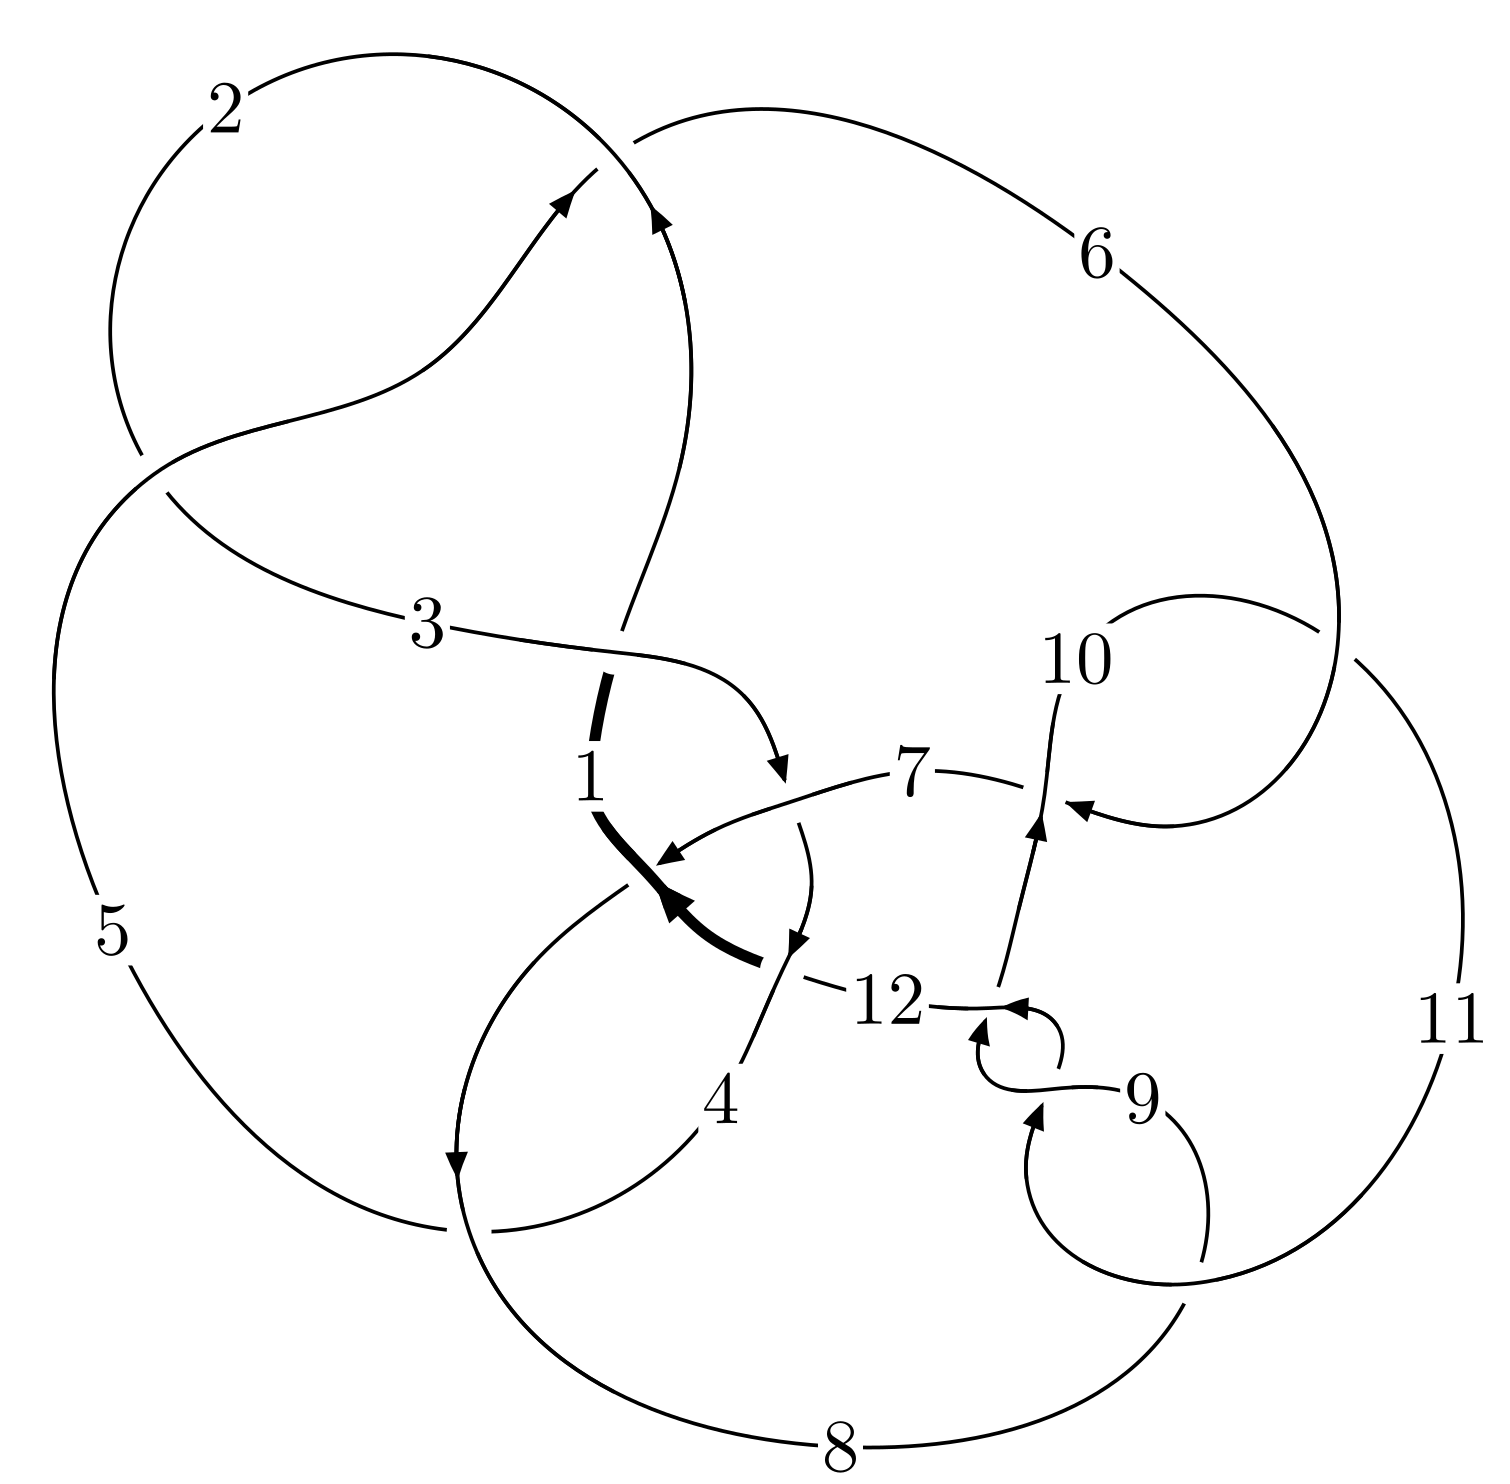
\includegraphics[width=112pt]{../../../GIT/diagram.site/Diagrams/png/868_12a_0067.png}\\
\ \ \ A knot diagram\footnotemark}&
\allowdisplaybreaks
\textbf{Linearized knot diagam} \\
\cline{2-2}
 &
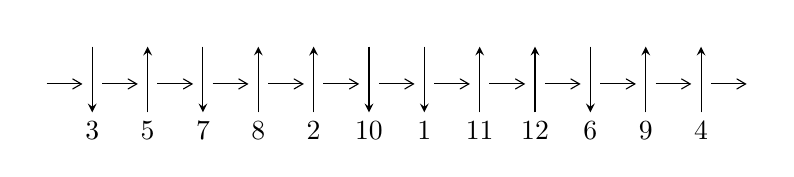
\begin{tikzpicture}[x=20pt, y=17pt]
	% nodes
	\node (C0) at (0, 0) {};
	\node (C1) at (1, 0) {};
	\node (C1U) at (1, +1) {};
	\node (C1D) at (1, -1) {3};

	\node (C2) at (2, 0) {};
	\node (C2U) at (2, +1) {};
	\node (C2D) at (2, -1) {5};

	\node (C3) at (3, 0) {};
	\node (C3U) at (3, +1) {};
	\node (C3D) at (3, -1) {7};

	\node (C4) at (4, 0) {};
	\node (C4U) at (4, +1) {};
	\node (C4D) at (4, -1) {8};

	\node (C5) at (5, 0) {};
	\node (C5U) at (5, +1) {};
	\node (C5D) at (5, -1) {2};

	\node (C6) at (6, 0) {};
	\node (C6U) at (6, +1) {};
	\node (C6D) at (6, -1) {10};

	\node (C7) at (7, 0) {};
	\node (C7U) at (7, +1) {};
	\node (C7D) at (7, -1) {1};

	\node (C8) at (8, 0) {};
	\node (C8U) at (8, +1) {};
	\node (C8D) at (8, -1) {11};

	\node (C9) at (9, 0) {};
	\node (C9U) at (9, +1) {};
	\node (C9D) at (9, -1) {12};

	\node (C10) at (10, 0) {};
	\node (C10U) at (10, +1) {};
	\node (C10D) at (10, -1) {6};

	\node (C11) at (11, 0) {};
	\node (C11U) at (11, +1) {};
	\node (C11D) at (11, -1) {9};

	\node (C12) at (12, 0) {};
	\node (C12U) at (12, +1) {};
	\node (C12D) at (12, -1) {4};
	\node (C13) at (13, 0) {};

	% arrows
	\draw[->,>={angle 60}]
	(C0) edge (C1) (C1) edge (C2) (C2) edge (C3) (C3) edge (C4) (C4) edge (C5) (C5) edge (C6) (C6) edge (C7) (C7) edge (C8) (C8) edge (C9) (C9) edge (C10) (C10) edge (C11) (C11) edge (C12) (C12) edge (C13) ;	\draw[->,>=stealth]
	(C1U) edge (C1D) (C2D) edge (C2U) (C3U) edge (C3D) (C4D) edge (C4U) (C5D) edge (C5U) (C6U) edge (C6D) (C7U) edge (C7D) (C8D) edge (C8U) (C9D) edge (C9U) (C10U) edge (C10D) (C11D) edge (C11U) (C12D) edge (C12U) ;
	\end{tikzpicture} \\
\hhline{~~} \\& 
\textbf{Solving Sequence} \\ \cline{2-2} 
 &
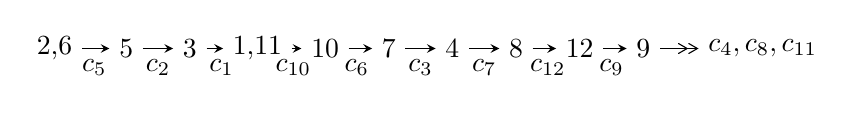
\begin{tikzpicture}[x=23pt, y=7pt]
	% node
	\node (A0) at (-1/8, 0) {2,6};
	\node (A1) at (1, 0) {5};
	\node (A2) at (2, 0) {3};
	\node (A3) at (49/16, 0) {1,11};
	\node (A4) at (33/8, 0) {10};
	\node (A5) at (41/8, 0) {7};
	\node (A6) at (49/8, 0) {4};
	\node (A7) at (57/8, 0) {8};
	\node (A8) at (65/8, 0) {12};
	\node (A9) at (73/8, 0) {9};
	\node (C1) at (1/2, -1) {$c_{5}$};
	\node (C2) at (3/2, -1) {$c_{2}$};
	\node (C3) at (5/2, -1) {$c_{1}$};
	\node (C4) at (29/8, -1) {$c_{10}$};
	\node (C5) at (37/8, -1) {$c_{6}$};
	\node (C6) at (45/8, -1) {$c_{3}$};
	\node (C7) at (53/8, -1) {$c_{7}$};
	\node (C8) at (61/8, -1) {$c_{12}$};
	\node (C9) at (69/8, -1) {$c_{9}$};
	\node (A10) at (11, 0) {$c_{4},c_{8},c_{11}$};

	% edge
	\draw[->,>=stealth]	
	(A0) edge (A1) (A1) edge (A2) (A2) edge (A3) (A3) edge (A4) (A4) edge (A5) (A5) edge (A6) (A6) edge (A7) (A7) edge (A8) (A8) edge (A9) ;
	\draw[->>,>={angle 60}]	
	(A9) edge (A10);
\end{tikzpicture} \\ 

\end{tabular} \\

\footnotetext{
The image of knot diagram is generated by the software ``\textbf{Draw programme}" developed by Andrew Bartholomew(\url{http://www.layer8.co.uk/maths/draw/index.htm\#Running-draw}), where we modified some parts for our purpose(\url{https://github.com/CATsTAILs/LinksPainter}).
}\phantom \\ \newline 
\centering \textbf{Ideals for irreducible components\footnotemark of $X_{\text{par}}$} 
 
\begin{align*}
I^u_{1}&=\langle 
-4.38800\times10^{265} u^{118}+3.02980\times10^{267} u^{117}+\cdots+1.78088\times10^{268} b-1.33871\times10^{268},\\
\phantom{I^u_{1}}&\phantom{= \langle  }-3.99262\times10^{266} u^{118}-9.19047\times10^{266} u^{117}+\cdots+4.68652\times10^{266} a-9.37332\times10^{266},\\
\phantom{I^u_{1}}&\phantom{= \langle  }u^{119}+2 u^{118}+\cdots+10 u-1\rangle \\
I^u_{2}&=\langle 
b,\;- u^3+a+2,\;u^4+u^2- u+1\rangle \\
I^u_{3}&=\langle 
b,\;- u^3- u^2+a-2 u-1,\;u^6+u^5+2 u^4+2 u^3+2 u^2+2 u+1\rangle \\
\\
\end{align*}
\raggedright * 3 irreducible components of $\dim_{\mathbb{C}}=0$, with total 129 representations.\\
\footnotetext{All coefficients of polynomials are rational numbers. But the coefficients are sometimes approximated in decimal forms when there is not enough margin.}
\newpage
\renewcommand{\arraystretch}{1}
\centering \section*{I. $I^u_{1}= \langle -4.39\times10^{265} u^{118}+3.03\times10^{267} u^{117}+\cdots+1.78\times10^{268} b-1.34\times10^{268},\;-3.99\times10^{266} u^{118}-9.19\times10^{266} u^{117}+\cdots+4.69\times10^{266} a-9.37\times10^{266},\;u^{119}+2 u^{118}+\cdots+10 u-1 \rangle$}
\flushleft \textbf{(i) Arc colorings}\\
\begin{tabular}{m{7pt} m{180pt} m{7pt} m{180pt} }
\flushright $a_{2}=$&$\begin{pmatrix}0\\u\end{pmatrix}$ \\
\flushright $a_{6}=$&$\begin{pmatrix}1\\0\end{pmatrix}$ \\
\flushright $a_{5}=$&$\begin{pmatrix}1\\u^2\end{pmatrix}$ \\
\flushright $a_{3}=$&$\begin{pmatrix}u\\u^3+u\end{pmatrix}$ \\
\flushright $a_{1}=$&$\begin{pmatrix}u^3\\u^5+u^3+u\end{pmatrix}$ \\
\flushright $a_{11}=$&$\begin{pmatrix}0.851939 u^{118}+1.96105 u^{117}+\cdots+5.50935 u+2.00006\\0.00246395 u^{118}-0.170130 u^{117}+\cdots-6.39561 u+0.751713\end{pmatrix}$ \\
\flushright $a_{10}=$&$\begin{pmatrix}0.854403 u^{118}+1.79092 u^{117}+\cdots-0.886258 u+2.75177\\0.00246395 u^{118}-0.170130 u^{117}+\cdots-6.39561 u+0.751713\end{pmatrix}$ \\
\flushright $a_{7}=$&$\begin{pmatrix}-1.38396 u^{118}-2.75797 u^{117}+\cdots+1.94382 u+0.347631\\0.656679 u^{118}+1.41118 u^{117}+\cdots-19.9698 u+2.06499\end{pmatrix}$ \\
\flushright $a_{4}=$&$\begin{pmatrix}0.330028 u^{118}+1.31635 u^{117}+\cdots+19.6110 u-6.37259\\-0.517151 u^{118}-0.974647 u^{117}+\cdots+15.4648 u-0.903539\end{pmatrix}$ \\
\flushright $a_{8}=$&$\begin{pmatrix}-1.41875 u^{118}-2.80068 u^{117}+\cdots+1.91552 u+0.343327\\0.587614 u^{118}+1.30438 u^{117}+\cdots-17.5478 u+1.69309\end{pmatrix}$ \\
\flushright $a_{12}=$&$\begin{pmatrix}-0.151740 u^{118}-0.172258 u^{117}+\cdots+0.396525 u-1.04773\\-0.132957 u^{118}-0.203298 u^{117}+\cdots+7.68780 u-0.734713\end{pmatrix}$ \\
\flushright $a_{9}=$&$\begin{pmatrix}0.448776 u^{118}+1.21621 u^{117}+\cdots-5.54442 u+2.77419\\0.132957 u^{118}+0.203298 u^{117}+\cdots-7.68780 u+0.734713\end{pmatrix}$\\&\end{tabular}
\flushleft \textbf{(ii) Obstruction class $= -1$}\\~\\
\flushleft \textbf{(iii) Cusp Shapes $= -0.699441 u^{118}-1.36103 u^{117}+\cdots-108.370 u+12.9128$}\\~\\
\newpage\renewcommand{\arraystretch}{1}
\flushleft \textbf{(iv) u-Polynomials at the component}\newline \\
\begin{tabular}{m{50pt}|m{274pt}}
Crossings & \hspace{64pt}u-Polynomials at each crossing \\
\hline $$\begin{aligned}c_{1}\end{aligned}$$&$\begin{aligned}
&u^{119}+48 u^{118}+\cdots+10 u-1
\end{aligned}$\\
\hline $$\begin{aligned}c_{2},c_{5}\end{aligned}$$&$\begin{aligned}
&u^{119}+2 u^{118}+\cdots+10 u-1
\end{aligned}$\\
\hline $$\begin{aligned}c_{3}\end{aligned}$$&$\begin{aligned}
&u^{119}+2 u^{118}+\cdots-140120 u+18392
\end{aligned}$\\
\hline $$\begin{aligned}c_{4}\end{aligned}$$&$\begin{aligned}
&u^{119}-2 u^{118}+\cdots+83530 u+30653
\end{aligned}$\\
\hline $$\begin{aligned}c_{6},c_{10}\end{aligned}$$&$\begin{aligned}
&u^{119}+u^{118}+\cdots+8192 u-1024
\end{aligned}$\\
\hline $$\begin{aligned}c_{7}\end{aligned}$$&$\begin{aligned}
&u^{119}-10 u^{118}+\cdots-2 u+1
\end{aligned}$\\
\hline $$\begin{aligned}c_{8},c_{9},c_{11}\end{aligned}$$&$\begin{aligned}
&u^{119}+11 u^{118}+\cdots-5 u-1
\end{aligned}$\\
\hline $$\begin{aligned}c_{12}\end{aligned}$$&$\begin{aligned}
&u^{119}+12 u^{118}+\cdots+2 u+1
\end{aligned}$\\
\hline
\end{tabular}\\~\\
\newpage\renewcommand{\arraystretch}{1}
\flushleft \textbf{(v) Riley Polynomials at the component}\newline \\
\begin{tabular}{m{50pt}|m{274pt}}
Crossings & \hspace{64pt}Riley Polynomials at each crossing \\
\hline $$\begin{aligned}c_{1}\end{aligned}$$&$\begin{aligned}
&y^{119}+48 y^{118}+\cdots+2322 y-1
\end{aligned}$\\
\hline $$\begin{aligned}c_{2},c_{5}\end{aligned}$$&$\begin{aligned}
&y^{119}+48 y^{118}+\cdots+10 y-1
\end{aligned}$\\
\hline $$\begin{aligned}c_{3}\end{aligned}$$&$\begin{aligned}
&y^{119}+132 y^{118}+\cdots-23236923728 y-338265664
\end{aligned}$\\
\hline $$\begin{aligned}c_{4}\end{aligned}$$&$\begin{aligned}
&y^{119}+108 y^{118}+\cdots-59171729182 y-939606409
\end{aligned}$\\
\hline $$\begin{aligned}c_{6},c_{10}\end{aligned}$$&$\begin{aligned}
&y^{119}+63 y^{118}+\cdots-16252928 y-1048576
\end{aligned}$\\
\hline $$\begin{aligned}c_{7}\end{aligned}$$&$\begin{aligned}
&y^{119}+12 y^{118}+\cdots-10 y-1
\end{aligned}$\\
\hline $$\begin{aligned}c_{8},c_{9},c_{11}\end{aligned}$$&$\begin{aligned}
&y^{119}-111 y^{118}+\cdots+61 y-1
\end{aligned}$\\
\hline $$\begin{aligned}c_{12}\end{aligned}$$&$\begin{aligned}
&y^{119}+120 y^{117}+\cdots+10 y-1
\end{aligned}$\\
\hline
\end{tabular}\\~\\
\newpage\flushleft \textbf{(vi) Complex Volumes and Cusp Shapes}
$$\begin{array}{c|c|c}  
\text{Solutions to }I^u_{1}& \I (\text{vol} + \sqrt{-1}CS) & \text{Cusp shape}\\
 \hline 
\begin{aligned}
u &= -0.838953 + 0.544196 I \\
a &= \phantom{-}0.109175 - 0.804084 I \\
b &= \phantom{-}0.227389 - 1.188850 I\end{aligned}
 & \phantom{-}4.58267 + 3.41945 I & \phantom{-0.000000 } 0 \\ \hline\begin{aligned}
u &= -0.838953 - 0.544196 I \\
a &= \phantom{-}0.109175 + 0.804084 I \\
b &= \phantom{-}0.227389 + 1.188850 I\end{aligned}
 & \phantom{-}4.58267 - 3.41945 I & \phantom{-0.000000 } 0 \\ \hline\begin{aligned}
u &= -0.566709 + 0.823835 I \\
a &= \phantom{-}1.41781 - 0.98974 I \\
b &= -1.49166 - 0.40339 I\end{aligned}
 & \phantom{-}4.10120 - 1.40763 I & \phantom{-0.000000 } 0 \\ \hline\begin{aligned}
u &= -0.566709 - 0.823835 I \\
a &= \phantom{-}1.41781 + 0.98974 I \\
b &= -1.49166 + 0.40339 I\end{aligned}
 & \phantom{-}4.10120 + 1.40763 I & \phantom{-0.000000 } 0 \\ \hline\begin{aligned}
u &= \phantom{-}0.929890 + 0.372568 I \\
a &= \phantom{-}0.494702 - 0.637233 I \\
b &= -0.186613 - 0.978134 I\end{aligned}
 & \phantom{-}3.57632 - 0.41841 I & \phantom{-0.000000 } 0 \\ \hline\begin{aligned}
u &= \phantom{-}0.929890 - 0.372568 I \\
a &= \phantom{-}0.494702 + 0.637233 I \\
b &= -0.186613 + 0.978134 I\end{aligned}
 & \phantom{-}3.57632 + 0.41841 I & \phantom{-0.000000 } 0 \\ \hline\begin{aligned}
u &= \phantom{-}0.528551 + 0.860721 I \\
a &= -1.65774 + 2.41316 I \\
b &= -0.856075 - 0.055946 I\end{aligned}
 & \phantom{-}2.60459 + 2.12994 I & \phantom{-0.000000 } 0 \\ \hline\begin{aligned}
u &= \phantom{-}0.528551 - 0.860721 I \\
a &= -1.65774 - 2.41316 I \\
b &= -0.856075 + 0.055946 I\end{aligned}
 & \phantom{-}2.60459 - 2.12994 I & \phantom{-0.000000 } 0 \\ \hline\begin{aligned}
u &= \phantom{-}0.429351 + 0.877830 I \\
a &= -0.87746 - 3.07903 I \\
b &= \phantom{-}0.391668 + 0.704858 I\end{aligned}
 & -0.147900 + 0.561296 I & \phantom{-0.000000 } 0 \\ \hline\begin{aligned}
u &= \phantom{-}0.429351 - 0.877830 I \\
a &= -0.87746 + 3.07903 I \\
b &= \phantom{-}0.391668 - 0.704858 I\end{aligned}
 & -0.147900 - 0.561296 I & \phantom{-0.000000 } 0\\
 \hline 
 \end{array}$$\newpage$$\begin{array}{c|c|c}  
\text{Solutions to }I^u_{1}& \I (\text{vol} + \sqrt{-1}CS) & \text{Cusp shape}\\
 \hline 
\begin{aligned}
u &= \phantom{-}0.595363 + 0.770782 I \\
a &= -0.47331 - 1.67093 I \\
b &= -0.426559 - 1.254360 I\end{aligned}
 & \phantom{-}6.60297 - 2.40686 I & \phantom{-0.000000 } 0 \\ \hline\begin{aligned}
u &= \phantom{-}0.595363 - 0.770782 I \\
a &= -0.47331 + 1.67093 I \\
b &= -0.426559 + 1.254360 I\end{aligned}
 & \phantom{-}6.60297 + 2.40686 I & \phantom{-0.000000 } 0 \\ \hline\begin{aligned}
u &= -0.886727 + 0.528667 I \\
a &= -0.901289 + 0.300957 I \\
b &= \phantom{-}1.234610 + 0.383617 I\end{aligned}
 & \phantom{-}5.90606 + 6.30718 I & \phantom{-0.000000 } 0 \\ \hline\begin{aligned}
u &= -0.886727 - 0.528667 I \\
a &= -0.901289 - 0.300957 I \\
b &= \phantom{-}1.234610 - 0.383617 I\end{aligned}
 & \phantom{-}5.90606 - 6.30718 I & \phantom{-0.000000 } 0 \\ \hline\begin{aligned}
u &= \phantom{-}0.518493 + 0.815351 I \\
a &= \phantom{-}0.25894 + 3.45551 I \\
b &= \phantom{-}0.260712 + 0.872493 I\end{aligned}
 & \phantom{-}0.677780 + 0.375001 I & \phantom{-0.000000 } 0 \\ \hline\begin{aligned}
u &= \phantom{-}0.518493 - 0.815351 I \\
a &= \phantom{-}0.25894 - 3.45551 I \\
b &= \phantom{-}0.260712 - 0.872493 I\end{aligned}
 & \phantom{-}0.677780 - 0.375001 I & \phantom{-0.000000 } 0 \\ \hline\begin{aligned}
u &= \phantom{-}0.356864 + 0.974923 I \\
a &= \phantom{-}0.19087 + 3.03439 I \\
b &= -0.382865 - 1.138070 I\end{aligned}
 & \phantom{-}4.96842 - 1.91691 I & \phantom{-0.000000 } 0 \\ \hline\begin{aligned}
u &= \phantom{-}0.356864 - 0.974923 I \\
a &= \phantom{-}0.19087 - 3.03439 I \\
b &= -0.382865 + 1.138070 I\end{aligned}
 & \phantom{-}4.96842 + 1.91691 I & \phantom{-0.000000 } 0 \\ \hline\begin{aligned}
u &= -0.575407 + 0.865942 I \\
a &= \phantom{-}0.67706 - 1.41907 I \\
b &= -1.38391 + 0.66586 I\end{aligned}
 & \phantom{-}3.96253 - 3.15795 I & \phantom{-0.000000 } 0 \\ \hline\begin{aligned}
u &= -0.575407 - 0.865942 I \\
a &= \phantom{-}0.67706 + 1.41907 I \\
b &= -1.38391 - 0.66586 I\end{aligned}
 & \phantom{-}3.96253 + 3.15795 I & \phantom{-0.000000 } 0\\
 \hline 
 \end{array}$$\newpage$$\begin{array}{c|c|c}  
\text{Solutions to }I^u_{1}& \I (\text{vol} + \sqrt{-1}CS) & \text{Cusp shape}\\
 \hline 
\begin{aligned}
u &= \phantom{-}0.526299 + 0.896866 I \\
a &= -4.03635 - 2.50678 I \\
b &= \phantom{-}0.356301 - 0.893080 I\end{aligned}
 & \phantom{-}0.40789 + 3.85492 I & \phantom{-0.000000 } 0 \\ \hline\begin{aligned}
u &= \phantom{-}0.526299 - 0.896866 I \\
a &= -4.03635 + 2.50678 I \\
b &= \phantom{-}0.356301 + 0.893080 I\end{aligned}
 & \phantom{-}0.40789 - 3.85492 I & \phantom{-0.000000 } 0 \\ \hline\begin{aligned}
u &= -0.913451 + 0.496996 I \\
a &= \phantom{-}0.431272 + 0.500496 I \\
b &= -0.520481 + 1.196970 I\end{aligned}
 & \phantom{-}3.03897 + 8.76012 I & \phantom{-0.000000 } 0 \\ \hline\begin{aligned}
u &= -0.913451 - 0.496996 I \\
a &= \phantom{-}0.431272 - 0.500496 I \\
b &= -0.520481 - 1.196970 I\end{aligned}
 & \phantom{-}3.03897 - 8.76012 I & \phantom{-0.000000 } 0 \\ \hline\begin{aligned}
u &= -0.555202 + 0.776269 I \\
a &= \phantom{-}1.94351 - 0.74037 I \\
b &= -0.651991 - 1.218550 I\end{aligned}
 & \phantom{-}3.14030 + 0.25233 I & \phantom{-0.000000 } 0 \\ \hline\begin{aligned}
u &= -0.555202 - 0.776269 I \\
a &= \phantom{-}1.94351 + 0.74037 I \\
b &= -0.651991 + 1.218550 I\end{aligned}
 & \phantom{-}3.14030 - 0.25233 I & \phantom{-0.000000 } 0 \\ \hline\begin{aligned}
u &= -0.311297 + 1.010080 I \\
a &= -0.730790 + 0.796137 I \\
b &= \phantom{-}0.720782 - 0.097822 I\end{aligned}
 & -3.66803 - 0.76142 I & \phantom{-0.000000 } 0 \\ \hline\begin{aligned}
u &= -0.311297 - 1.010080 I \\
a &= -0.730790 - 0.796137 I \\
b &= \phantom{-}0.720782 + 0.097822 I\end{aligned}
 & -3.66803 + 0.76142 I & \phantom{-0.000000 } 0 \\ \hline\begin{aligned}
u &= \phantom{-}0.494555 + 0.800584 I \\
a &= \phantom{-}4.89193 - 0.43239 I \\
b &= -0.486675 + 0.231669 I\end{aligned}
 & \phantom{-}2.15098 + 1.56600 I & \phantom{-0.000000 } 0 \\ \hline\begin{aligned}
u &= \phantom{-}0.494555 - 0.800584 I \\
a &= \phantom{-}4.89193 + 0.43239 I \\
b &= -0.486675 - 0.231669 I\end{aligned}
 & \phantom{-}2.15098 - 1.56600 I & \phantom{-0.000000 } 0\\
 \hline 
 \end{array}$$\newpage$$\begin{array}{c|c|c}  
\text{Solutions to }I^u_{1}& \I (\text{vol} + \sqrt{-1}CS) & \text{Cusp shape}\\
 \hline 
\begin{aligned}
u &= \phantom{-}0.442347 + 0.967147 I \\
a &= \phantom{-}0.187163 + 0.721442 I \\
b &= \phantom{-}0.203483 - 0.360440 I\end{aligned}
 & -0.42288 + 2.75298 I & \phantom{-0.000000 } 0 \\ \hline\begin{aligned}
u &= \phantom{-}0.442347 - 0.967147 I \\
a &= \phantom{-}0.187163 - 0.721442 I \\
b &= \phantom{-}0.203483 + 0.360440 I\end{aligned}
 & -0.42288 - 2.75298 I & \phantom{-0.000000 } 0 \\ \hline\begin{aligned}
u &= -0.098695 + 0.931045 I \\
a &= \phantom{-}0.77161 - 1.97635 I \\
b &= -0.628406 + 1.083000 I\end{aligned}
 & \phantom{-}3.41353 + 5.41155 I & \phantom{-0.000000 } 0 \\ \hline\begin{aligned}
u &= -0.098695 - 0.931045 I \\
a &= \phantom{-}0.77161 + 1.97635 I \\
b &= -0.628406 - 1.083000 I\end{aligned}
 & \phantom{-}3.41353 - 5.41155 I & \phantom{-0.000000 } 0 \\ \hline\begin{aligned}
u &= \phantom{-}0.951835 + 0.487655 I \\
a &= -1.263630 + 0.008890 I \\
b &= \phantom{-}1.025210 + 0.046098 I\end{aligned}
 & \phantom{-}5.49536 + 1.71804 I & \phantom{-0.000000 } 0 \\ \hline\begin{aligned}
u &= \phantom{-}0.951835 - 0.487655 I \\
a &= -1.263630 - 0.008890 I \\
b &= \phantom{-}1.025210 - 0.046098 I\end{aligned}
 & \phantom{-}5.49536 - 1.71804 I & \phantom{-0.000000 } 0 \\ \hline\begin{aligned}
u &= -0.578907 + 0.899689 I \\
a &= -0.491377 - 0.195288 I \\
b &= -0.40200 + 1.40800 I\end{aligned}
 & \phantom{-}2.74244 - 4.81471 I & \phantom{-0.000000 } 0 \\ \hline\begin{aligned}
u &= -0.578907 - 0.899689 I \\
a &= -0.491377 + 0.195288 I \\
b &= -0.40200 - 1.40800 I\end{aligned}
 & \phantom{-}2.74244 + 4.81471 I & \phantom{-0.000000 } 0 \\ \hline\begin{aligned}
u &= \phantom{-}0.557211 + 0.926119 I \\
a &= \phantom{-}2.25509 - 2.77223 I \\
b &= -0.148264 - 0.425639 I\end{aligned}
 & \phantom{-}1.67285 + 2.69563 I & \phantom{-0.000000 } 0 \\ \hline\begin{aligned}
u &= \phantom{-}0.557211 - 0.926119 I \\
a &= \phantom{-}2.25509 + 2.77223 I \\
b &= -0.148264 + 0.425639 I\end{aligned}
 & \phantom{-}1.67285 - 2.69563 I & \phantom{-0.000000 } 0\\
 \hline 
 \end{array}$$\newpage$$\begin{array}{c|c|c}  
\text{Solutions to }I^u_{1}& \I (\text{vol} + \sqrt{-1}CS) & \text{Cusp shape}\\
 \hline 
\begin{aligned}
u &= -0.561845 + 0.934937 I \\
a &= -2.05105 + 0.47513 I \\
b &= \phantom{-}0.64960 + 1.35081 I\end{aligned}
 & \phantom{-}0.66033 - 5.93367 I & \phantom{-0.000000 } 0 \\ \hline\begin{aligned}
u &= -0.561845 - 0.934937 I \\
a &= -2.05105 - 0.47513 I \\
b &= \phantom{-}0.64960 - 1.35081 I\end{aligned}
 & \phantom{-}0.66033 + 5.93367 I & \phantom{-0.000000 } 0 \\ \hline\begin{aligned}
u &= \phantom{-}0.567410 + 0.933478 I \\
a &= \phantom{-}3.34553 + 1.33510 I \\
b &= -0.498602 + 1.231420 I\end{aligned}
 & \phantom{-}6.08874 + 7.00877 I & \phantom{-0.000000 } 0 \\ \hline\begin{aligned}
u &= \phantom{-}0.567410 - 0.933478 I \\
a &= \phantom{-}3.34553 - 1.33510 I \\
b &= -0.498602 - 1.231420 I\end{aligned}
 & \phantom{-}6.08874 - 7.00877 I & \phantom{-0.000000 } 0 \\ \hline\begin{aligned}
u &= -0.976182 + 0.493516 I \\
a &= -0.586235 - 0.134004 I \\
b &= \phantom{-}0.71252 - 1.31592 I\end{aligned}
 & \phantom{-}8.9345 + 13.2205 I & \phantom{-0.000000 } 0 \\ \hline\begin{aligned}
u &= -0.976182 - 0.493516 I \\
a &= -0.586235 + 0.134004 I \\
b &= \phantom{-}0.71252 + 1.31592 I\end{aligned}
 & \phantom{-}8.9345 - 13.2205 I & \phantom{-0.000000 } 0 \\ \hline\begin{aligned}
u &= -0.837165 + 0.713055 I \\
a &= -0.907014 + 0.200119 I \\
b &= \phantom{-}0.10091 + 1.56443 I\end{aligned}
 & \phantom{-}13.31560 + 1.26216 I & \phantom{-0.000000 } 0 \\ \hline\begin{aligned}
u &= -0.837165 - 0.713055 I \\
a &= -0.907014 - 0.200119 I \\
b &= \phantom{-}0.10091 - 1.56443 I\end{aligned}
 & \phantom{-}13.31560 - 1.26216 I & \phantom{-0.000000 } 0 \\ \hline\begin{aligned}
u &= -0.511882 + 0.735751 I \\
a &= \phantom{-}0.633141 - 0.149979 I \\
b &= \phantom{-}0.39152 - 1.36600 I\end{aligned}
 & \phantom{-}1.31767 + 1.52824 I & \phantom{-0.000000 } 0 \\ \hline\begin{aligned}
u &= -0.511882 - 0.735751 I \\
a &= \phantom{-}0.633141 + 0.149979 I \\
b &= \phantom{-}0.39152 + 1.36600 I\end{aligned}
 & \phantom{-}1.31767 - 1.52824 I & \phantom{-0.000000 } 0\\
 \hline 
 \end{array}$$\newpage$$\begin{array}{c|c|c}  
\text{Solutions to }I^u_{1}& \I (\text{vol} + \sqrt{-1}CS) & \text{Cusp shape}\\
 \hline 
\begin{aligned}
u &= -0.783521 + 0.422905 I \\
a &= \phantom{-}0.486131 - 0.247012 I \\
b &= -0.755611 - 0.251969 I\end{aligned}
 & \phantom{-}0.15512 + 3.88915 I & \phantom{-0.000000 } 0 \\ \hline\begin{aligned}
u &= -0.783521 - 0.422905 I \\
a &= \phantom{-}0.486131 + 0.247012 I \\
b &= -0.755611 + 0.251969 I\end{aligned}
 & \phantom{-}0.15512 - 3.88915 I & \phantom{-0.000000 } 0 \\ \hline\begin{aligned}
u &= -0.652570 + 0.596164 I \\
a &= -0.0981409 + 0.0613103 I \\
b &= -0.68690 + 1.37885 I\end{aligned}
 & \phantom{-}7.74142 + 6.02428 I & \phantom{-0.000000 } 0 \\ \hline\begin{aligned}
u &= -0.652570 - 0.596164 I \\
a &= -0.0981409 - 0.0613103 I \\
b &= -0.68690 - 1.37885 I\end{aligned}
 & \phantom{-}7.74142 - 6.02428 I & \phantom{-0.000000 } 0 \\ \hline\begin{aligned}
u &= \phantom{-}0.952391 + 0.588335 I \\
a &= \phantom{-}0.591023 + 0.694941 I \\
b &= -0.270109 + 1.002650 I\end{aligned}
 & \phantom{-}3.36143 + 3.82787 I & \phantom{-0.000000 } 0 \\ \hline\begin{aligned}
u &= \phantom{-}0.952391 - 0.588335 I \\
a &= \phantom{-}0.591023 - 0.694941 I \\
b &= -0.270109 - 1.002650 I\end{aligned}
 & \phantom{-}3.36143 - 3.82787 I & \phantom{-0.000000 } 0 \\ \hline\begin{aligned}
u &= \phantom{-}0.017038 + 1.121140 I \\
a &= -0.763804 + 0.103402 I \\
b &= \phantom{-}0.392618 - 0.845484 I\end{aligned}
 & -1.51868 + 2.01224 I & \phantom{-0.000000 } 0 \\ \hline\begin{aligned}
u &= \phantom{-}0.017038 - 1.121140 I \\
a &= -0.763804 - 0.103402 I \\
b &= \phantom{-}0.392618 + 0.845484 I\end{aligned}
 & -1.51868 - 2.01224 I & \phantom{-0.000000 } 0 \\ \hline\begin{aligned}
u &= -0.522097 + 1.002300 I \\
a &= -1.43550 + 0.42911 I \\
b &= \phantom{-}1.002750 + 0.439220 I\end{aligned}
 & -2.32372 - 5.35556 I & \phantom{-0.000000 } 0 \\ \hline\begin{aligned}
u &= -0.522097 - 1.002300 I \\
a &= -1.43550 - 0.42911 I \\
b &= \phantom{-}1.002750 - 0.439220 I\end{aligned}
 & -2.32372 + 5.35556 I & \phantom{-0.000000 } 0\\
 \hline 
 \end{array}$$\newpage$$\begin{array}{c|c|c}  
\text{Solutions to }I^u_{1}& \I (\text{vol} + \sqrt{-1}CS) & \text{Cusp shape}\\
 \hline 
\begin{aligned}
u &= \phantom{-}1.109750 + 0.291509 I \\
a &= -0.578286 - 0.115750 I \\
b &= \phantom{-}0.431413 + 1.312020 I\end{aligned}
 & \phantom{-}9.92813 - 3.32978 I & \phantom{-0.000000 } 0 \\ \hline\begin{aligned}
u &= \phantom{-}1.109750 - 0.291509 I \\
a &= -0.578286 + 0.115750 I \\
b &= \phantom{-}0.431413 - 1.312020 I\end{aligned}
 & \phantom{-}9.92813 + 3.32978 I & \phantom{-0.000000 } 0 \\ \hline\begin{aligned}
u &= \phantom{-}0.618376 + 0.563906 I \\
a &= \phantom{-}0.730085 - 0.169336 I \\
b &= -0.337347 - 0.043445 I\end{aligned}
 & \phantom{-}1.11265 + 1.43327 I & \phantom{-0.000000 } 0 \\ \hline\begin{aligned}
u &= \phantom{-}0.618376 - 0.563906 I \\
a &= \phantom{-}0.730085 + 0.169336 I \\
b &= -0.337347 + 0.043445 I\end{aligned}
 & \phantom{-}1.11265 - 1.43327 I & \phantom{-0.000000 } 0 \\ \hline\begin{aligned}
u &= -0.615027 + 1.005040 I \\
a &= \phantom{-}2.23322 - 0.35155 I \\
b &= -0.81135 - 1.33905 I\end{aligned}
 & \phantom{-}6.53771 - 10.99580 I & \phantom{-0.000000 } 0 \\ \hline\begin{aligned}
u &= -0.615027 - 1.005040 I \\
a &= \phantom{-}2.23322 + 0.35155 I \\
b &= -0.81135 + 1.33905 I\end{aligned}
 & \phantom{-}6.53771 + 10.99580 I & \phantom{-0.000000 } 0 \\ \hline\begin{aligned}
u &= -0.106450 + 1.175170 I \\
a &= \phantom{-}1.60470 + 0.24304 I \\
b &= -0.708952 - 0.522934 I\end{aligned}
 & -5.13196 + 1.58072 I & \phantom{-0.000000 } 0 \\ \hline\begin{aligned}
u &= -0.106450 - 1.175170 I \\
a &= \phantom{-}1.60470 - 0.24304 I \\
b &= -0.708952 + 0.522934 I\end{aligned}
 & -5.13196 - 1.58072 I & \phantom{-0.000000 } 0 \\ \hline\begin{aligned}
u &= -0.322092 + 0.754108 I \\
a &= -0.39118 + 1.39798 I \\
b &= \phantom{-}0.803778 - 0.818065 I\end{aligned}
 & -1.06689 + 1.52634 I & \phantom{-0.000000 } 0 \\ \hline\begin{aligned}
u &= -0.322092 - 0.754108 I \\
a &= -0.39118 - 1.39798 I \\
b &= \phantom{-}0.803778 + 0.818065 I\end{aligned}
 & -1.06689 - 1.52634 I & \phantom{-0.000000 } 0\\
 \hline 
 \end{array}$$\newpage$$\begin{array}{c|c|c}  
\text{Solutions to }I^u_{1}& \I (\text{vol} + \sqrt{-1}CS) & \text{Cusp shape}\\
 \hline 
\begin{aligned}
u &= -0.803859 + 0.148657 I \\
a &= -0.225213 - 0.234367 I \\
b &= -0.064271 + 0.891155 I\end{aligned}
 & \phantom{-}2.46591 + 3.13553 I & \phantom{-0.000000 } 0 \\ \hline\begin{aligned}
u &= -0.803859 - 0.148657 I \\
a &= -0.225213 + 0.234367 I \\
b &= -0.064271 - 0.891155 I\end{aligned}
 & \phantom{-}2.46591 - 3.13553 I & \phantom{-0.000000 } 0 \\ \hline\begin{aligned}
u &= \phantom{-}0.520708 + 1.090110 I \\
a &= \phantom{-}0.693612 + 0.589861 I \\
b &= -0.366092 - 0.404737 I\end{aligned}
 & -0.47565 + 2.99344 I & \phantom{-0.000000 } 0 \\ \hline\begin{aligned}
u &= \phantom{-}0.520708 - 1.090110 I \\
a &= \phantom{-}0.693612 - 0.589861 I \\
b &= -0.366092 + 0.404737 I\end{aligned}
 & -0.47565 - 2.99344 I & \phantom{-0.000000 } 0 \\ \hline\begin{aligned}
u &= \phantom{-}0.058363 + 1.216070 I \\
a &= -2.32308 - 0.15998 I \\
b &= \phantom{-}0.971579 + 0.429480 I\end{aligned}
 & -0.70650 + 4.43937 I & \phantom{-0.000000 } 0 \\ \hline\begin{aligned}
u &= \phantom{-}0.058363 - 1.216070 I \\
a &= -2.32308 + 0.15998 I \\
b &= \phantom{-}0.971579 - 0.429480 I\end{aligned}
 & -0.70650 - 4.43937 I & \phantom{-0.000000 } 0 \\ \hline\begin{aligned}
u &= -0.727403 + 0.981872 I \\
a &= \phantom{-}1.071830 + 0.200891 I \\
b &= -0.01760 - 1.62299 I\end{aligned}
 & \phantom{-}12.4827 - 7.0839 I & \phantom{-0.000000 } 0 \\ \hline\begin{aligned}
u &= -0.727403 - 0.981872 I \\
a &= \phantom{-}1.071830 - 0.200891 I \\
b &= -0.01760 + 1.62299 I\end{aligned}
 & \phantom{-}12.4827 + 7.0839 I & \phantom{-0.000000 } 0 \\ \hline\begin{aligned}
u &= -0.612589 + 1.094200 I \\
a &= \phantom{-}0.767693 - 0.894702 I \\
b &= -0.892482 + 0.262426 I\end{aligned}
 & -1.81583 - 9.13295 I & \phantom{-0.000000 } 0 \\ \hline\begin{aligned}
u &= -0.612589 - 1.094200 I \\
a &= \phantom{-}0.767693 + 0.894702 I \\
b &= -0.892482 - 0.262426 I\end{aligned}
 & -1.81583 + 9.13295 I & \phantom{-0.000000 } 0\\
 \hline 
 \end{array}$$\newpage$$\begin{array}{c|c|c}  
\text{Solutions to }I^u_{1}& \I (\text{vol} + \sqrt{-1}CS) & \text{Cusp shape}\\
 \hline 
\begin{aligned}
u &= \phantom{-}0.735041 + 1.019170 I \\
a &= -0.316372 - 0.656191 I \\
b &= -0.077697 - 0.865759 I\end{aligned}
 & \phantom{-}2.05334 + 2.32542 I & \phantom{-0.000000 } 0 \\ \hline\begin{aligned}
u &= \phantom{-}0.735041 - 1.019170 I \\
a &= -0.316372 + 0.656191 I \\
b &= -0.077697 + 0.865759 I\end{aligned}
 & \phantom{-}2.05334 - 2.32542 I & \phantom{-0.000000 } 0 \\ \hline\begin{aligned}
u &= -0.518341 + 1.151770 I \\
a &= \phantom{-}0.645899 + 0.752822 I \\
b &= -0.126191 - 0.699313 I\end{aligned}
 & -0.44007 - 7.88693 I & \phantom{-0.000000 } 0 \\ \hline\begin{aligned}
u &= -0.518341 - 1.151770 I \\
a &= \phantom{-}0.645899 - 0.752822 I \\
b &= -0.126191 + 0.699313 I\end{aligned}
 & -0.44007 + 7.88693 I & \phantom{-0.000000 } 0 \\ \hline\begin{aligned}
u &= \phantom{-}1.082210 + 0.653636 I \\
a &= -0.837140 - 0.100407 I \\
b &= \phantom{-}0.485630 - 1.303600 I\end{aligned}
 & \phantom{-}9.53931 + 7.04970 I & \phantom{-0.000000 } 0 \\ \hline\begin{aligned}
u &= \phantom{-}1.082210 - 0.653636 I \\
a &= -0.837140 + 0.100407 I \\
b &= \phantom{-}0.485630 + 1.303600 I\end{aligned}
 & \phantom{-}9.53931 - 7.04970 I & \phantom{-0.000000 } 0 \\ \hline\begin{aligned}
u &= -0.285135 + 1.235900 I \\
a &= -0.837715 - 1.017010 I \\
b &= \phantom{-}0.191982 + 0.843692 I\end{aligned}
 & -1.96720 - 0.65100 I & \phantom{-0.000000 } 0 \\ \hline\begin{aligned}
u &= -0.285135 - 1.235900 I \\
a &= -0.837715 + 1.017010 I \\
b &= \phantom{-}0.191982 - 0.843692 I\end{aligned}
 & -1.96720 + 0.65100 I & \phantom{-0.000000 } 0 \\ \hline\begin{aligned}
u &= -0.670191 + 1.077940 I \\
a &= -1.54529 + 0.46264 I \\
b &= \phantom{-}0.332562 + 1.244600 I\end{aligned}
 & \phantom{-}2.96632 - 9.05048 I & \phantom{-0.000000 } 0 \\ \hline\begin{aligned}
u &= -0.670191 - 1.077940 I \\
a &= -1.54529 - 0.46264 I \\
b &= \phantom{-}0.332562 - 1.244600 I\end{aligned}
 & \phantom{-}2.96632 + 9.05048 I & \phantom{-0.000000 } 0\\
 \hline 
 \end{array}$$\newpage$$\begin{array}{c|c|c}  
\text{Solutions to }I^u_{1}& \I (\text{vol} + \sqrt{-1}CS) & \text{Cusp shape}\\
 \hline 
\begin{aligned}
u &= \phantom{-}0.022366 + 1.275070 I \\
a &= \phantom{-}1.23684 - 0.76817 I \\
b &= -0.545853 + 1.021420 I\end{aligned}
 & -3.60584 + 6.39853 I & \phantom{-0.000000 } 0 \\ \hline\begin{aligned}
u &= \phantom{-}0.022366 - 1.275070 I \\
a &= \phantom{-}1.23684 + 0.76817 I \\
b &= -0.545853 - 1.021420 I\end{aligned}
 & -3.60584 - 6.39853 I & \phantom{-0.000000 } 0 \\ \hline\begin{aligned}
u &= -0.683411 + 1.099690 I \\
a &= -1.00098 + 1.27401 I \\
b &= \phantom{-}1.272770 - 0.469310 I\end{aligned}
 & \phantom{-}4.16552 - 12.10780 I & \phantom{-0.000000 } 0 \\ \hline\begin{aligned}
u &= -0.683411 - 1.099690 I \\
a &= -1.00098 - 1.27401 I \\
b &= \phantom{-}1.272770 + 0.469310 I\end{aligned}
 & \phantom{-}4.16552 + 12.10780 I & \phantom{-0.000000 } 0 \\ \hline\begin{aligned}
u &= -0.681332 + 1.121330 I \\
a &= \phantom{-}1.99277 - 0.41746 I \\
b &= -0.585302 - 1.226580 I\end{aligned}
 & \phantom{-}1.1322 - 14.6195 I & \phantom{-0.000000 } 0 \\ \hline\begin{aligned}
u &= -0.681332 - 1.121330 I \\
a &= \phantom{-}1.99277 + 0.41746 I \\
b &= -0.585302 + 1.226580 I\end{aligned}
 & \phantom{-}1.1322 + 14.6195 I & \phantom{-0.000000 } 0 \\ \hline\begin{aligned}
u &= \phantom{-}0.720492 + 1.113940 I \\
a &= -1.51475 - 0.74596 I \\
b &= \phantom{-}0.982362 + 0.178327 I\end{aligned}
 & \phantom{-}3.61125 + 4.38522 I & \phantom{-0.000000 } 0 \\ \hline\begin{aligned}
u &= \phantom{-}0.720492 - 1.113940 I \\
a &= -1.51475 + 0.74596 I \\
b &= \phantom{-}0.982362 - 0.178327 I\end{aligned}
 & \phantom{-}3.61125 - 4.38522 I & \phantom{-0.000000 } 0 \\ \hline\begin{aligned}
u &= -0.701138 + 1.147870 I \\
a &= -2.22521 + 0.22453 I \\
b &= \phantom{-}0.76422 + 1.30680 I\end{aligned}
 & \phantom{-}6.9107 - 19.3213 I & \phantom{-0.000000 } 0 \\ \hline\begin{aligned}
u &= -0.701138 - 1.147870 I \\
a &= -2.22521 - 0.22453 I \\
b &= \phantom{-}0.76422 - 1.30680 I\end{aligned}
 & \phantom{-}6.9107 + 19.3213 I & \phantom{-0.000000 } 0\\
 \hline 
 \end{array}$$\newpage$$\begin{array}{c|c|c}  
\text{Solutions to }I^u_{1}& \I (\text{vol} + \sqrt{-1}CS) & \text{Cusp shape}\\
 \hline 
\begin{aligned}
u &= \phantom{-}0.693659 + 1.171160 I \\
a &= \phantom{-}1.59038 + 0.32423 I \\
b &= -0.382587 + 1.003640 I\end{aligned}
 & \phantom{-}1.19440 + 6.39011 I & \phantom{-0.000000 } 0 \\ \hline\begin{aligned}
u &= \phantom{-}0.693659 - 1.171160 I \\
a &= \phantom{-}1.59038 - 0.32423 I \\
b &= -0.382587 - 1.003640 I\end{aligned}
 & \phantom{-}1.19440 - 6.39011 I & \phantom{-0.000000 } 0 \\ \hline\begin{aligned}
u &= \phantom{-}0.035679 + 1.363720 I \\
a &= -1.36652 + 1.22183 I \\
b &= \phantom{-}0.638039 - 1.211900 I\end{aligned}
 & \phantom{-}1.81121 + 10.37090 I & \phantom{-0.000000 } 0 \\ \hline\begin{aligned}
u &= \phantom{-}0.035679 - 1.363720 I \\
a &= -1.36652 - 1.22183 I \\
b &= \phantom{-}0.638039 + 1.211900 I\end{aligned}
 & \phantom{-}1.81121 - 10.37090 I & \phantom{-0.000000 } 0 \\ \hline\begin{aligned}
u &= \phantom{-}0.388544 + 1.308910 I \\
a &= -0.21975 - 1.45578 I \\
b &= \phantom{-}0.271184 + 1.181390 I\end{aligned}
 & \phantom{-}4.63253 + 1.58055 I & \phantom{-0.000000 } 0 \\ \hline\begin{aligned}
u &= \phantom{-}0.388544 - 1.308910 I \\
a &= -0.21975 + 1.45578 I \\
b &= \phantom{-}0.271184 - 1.181390 I\end{aligned}
 & \phantom{-}4.63253 - 1.58055 I & \phantom{-0.000000 } 0 \\ \hline\begin{aligned}
u &= \phantom{-}0.906319 + 1.043070 I \\
a &= \phantom{-}0.150159 - 0.428837 I \\
b &= \phantom{-}0.364395 + 1.282450 I\end{aligned}
 & \phantom{-}8.37474 - 0.01682 I & \phantom{-0.000000 } 0 \\ \hline\begin{aligned}
u &= \phantom{-}0.906319 - 1.043070 I \\
a &= \phantom{-}0.150159 + 0.428837 I \\
b &= \phantom{-}0.364395 - 1.282450 I\end{aligned}
 & \phantom{-}8.37474 + 0.01682 I & \phantom{-0.000000 } 0 \\ \hline\begin{aligned}
u &= \phantom{-}0.73537 + 1.25030 I \\
a &= -1.76430 + 0.25295 I \\
b &= \phantom{-}0.545981 - 1.269200 I\end{aligned}
 & \phantom{-}7.05259 + 9.90887 I & \phantom{-0.000000 } 0 \\ \hline\begin{aligned}
u &= \phantom{-}0.73537 - 1.25030 I \\
a &= -1.76430 - 0.25295 I \\
b &= \phantom{-}0.545981 + 1.269200 I\end{aligned}
 & \phantom{-}7.05259 - 9.90887 I & \phantom{-0.000000 } 0\\
 \hline 
 \end{array}$$\newpage$$\begin{array}{c|c|c}  
\text{Solutions to }I^u_{1}& \I (\text{vol} + \sqrt{-1}CS) & \text{Cusp shape}\\
 \hline 
\begin{aligned}
u &= \phantom{-}0.412631 + 0.283829 I \\
a &= -0.447411 - 0.881091 I \\
b &= -0.455410 + 1.286190 I\end{aligned}
 & \phantom{-}6.81704 + 5.01481 I & \phantom{-}2.95424 - 4.27680 I \\ \hline\begin{aligned}
u &= \phantom{-}0.412631 - 0.283829 I \\
a &= -0.447411 + 0.881091 I \\
b &= -0.455410 - 1.286190 I\end{aligned}
 & \phantom{-}6.81704 - 5.01481 I & \phantom{-}2.95424 + 4.27680 I \\ \hline\begin{aligned}
u &= -0.332585 + 0.209939 I \\
a &= \phantom{-}1.001600 + 0.735256 I \\
b &= \phantom{-}0.599999 - 0.527709 I\end{aligned}
 & -0.78514 + 1.51036 I & -1.09782 - 4.16173 I \\ \hline\begin{aligned}
u &= -0.332585 - 0.209939 I \\
a &= \phantom{-}1.001600 - 0.735256 I \\
b &= \phantom{-}0.599999 + 0.527709 I\end{aligned}
 & -0.78514 - 1.51036 I & -1.09782 + 4.16173 I \\ \hline\begin{aligned}
u &= \phantom{-}0.144570 + 0.213517 I \\
a &= \phantom{-}5.52126 - 0.96142 I \\
b &= -0.480746 - 0.462220 I\end{aligned}
 & \phantom{-}2.12966 + 0.82300 I & \phantom{-}5.18127 + 1.42411 I \\ \hline\begin{aligned}
u &= \phantom{-}0.144570 - 0.213517 I \\
a &= \phantom{-}5.52126 + 0.96142 I \\
b &= -0.480746 + 0.462220 I\end{aligned}
 & \phantom{-}2.12966 - 0.82300 I & \phantom{-}5.18127 - 1.42411 I \\ \hline\begin{aligned}
u &= \phantom{-}0.111732 + 0.194107 I \\
a &= \phantom{-}2.24806 + 1.10571 I \\
b &= \phantom{-}0.275565 - 0.965943 I\end{aligned}
 & \phantom{-}0.69537 + 1.96234 I & \phantom{-}0.92100 - 4.57588 I \\ \hline\begin{aligned}
u &= \phantom{-}0.111732 - 0.194107 I \\
a &= \phantom{-}2.24806 - 1.10571 I \\
b &= \phantom{-}0.275565 + 0.965943 I\end{aligned}
 & \phantom{-}0.69537 - 1.96234 I & \phantom{-}0.92100 + 4.57588 I \\ \hline\begin{aligned}
u &= \phantom{-}0.133516\phantom{ +0.000000I} \\
a &= \phantom{-}6.38767\phantom{ +0.000000I} \\
b &= -0.945861\phantom{ +0.000000I}\end{aligned}
 & \phantom{-}2.76788\phantom{ +0.000000I} & \phantom{-}1.73080\phantom{ +0.000000I}\\
 \hline 
 \end{array}$$\newpage\newpage\renewcommand{\arraystretch}{1}
\centering \section*{II. $I^u_{2}= \langle b,\;- u^3+a+2,\;u^4+u^2- u+1 \rangle$}
\flushleft \textbf{(i) Arc colorings}\\
\begin{tabular}{m{7pt} m{180pt} m{7pt} m{180pt} }
\flushright $a_{2}=$&$\begin{pmatrix}0\\u\end{pmatrix}$ \\
\flushright $a_{6}=$&$\begin{pmatrix}1\\0\end{pmatrix}$ \\
\flushright $a_{5}=$&$\begin{pmatrix}1\\u^2\end{pmatrix}$ \\
\flushright $a_{3}=$&$\begin{pmatrix}u\\u^3+u\end{pmatrix}$ \\
\flushright $a_{1}=$&$\begin{pmatrix}u^3\\u^2\end{pmatrix}$ \\
\flushright $a_{11}=$&$\begin{pmatrix}u^3-2\\0\end{pmatrix}$ \\
\flushright $a_{10}=$&$\begin{pmatrix}u^3-2\\0\end{pmatrix}$ \\
\flushright $a_{7}=$&$\begin{pmatrix}1\\0\end{pmatrix}$ \\
\flushright $a_{4}=$&$\begin{pmatrix}- u^3\\u^3+u\end{pmatrix}$ \\
\flushright $a_{8}=$&$\begin{pmatrix}- u^3+u^2- u+1\\- u^2+u-1\end{pmatrix}$ \\
\flushright $a_{12}=$&$\begin{pmatrix}u^3- u^2+u-1\\u^2- u+1\end{pmatrix}$ \\
\flushright $a_{9}=$&$\begin{pmatrix}u^2- u-1\\- u^2+u-1\end{pmatrix}$\\&\end{tabular}
\flushleft \textbf{(ii) Obstruction class $= 1$}\\~\\
\flushleft \textbf{(iii) Cusp Shapes $= -9 u^3-2 u^2-2 u+11$}\\~\\
\newpage\renewcommand{\arraystretch}{1}
\flushleft \textbf{(iv) u-Polynomials at the component}\newline \\
\begin{tabular}{m{50pt}|m{274pt}}
Crossings & \hspace{64pt}u-Polynomials at each crossing \\
\hline $$\begin{aligned}c_{1}\end{aligned}$$&$\begin{aligned}
&u^4-2 u^3+3 u^2- u+1
\end{aligned}$\\
\hline $$\begin{aligned}c_{2},c_{4},c_{12}\end{aligned}$$&$\begin{aligned}
&u^4+u^2+u+1
\end{aligned}$\\
\hline $$\begin{aligned}c_{3}\end{aligned}$$&$\begin{aligned}
&u^4+3 u^3+4 u^2+3 u+2
\end{aligned}$\\
\hline $$\begin{aligned}c_{5}\end{aligned}$$&$\begin{aligned}
&u^4+u^2- u+1
\end{aligned}$\\
\hline $$\begin{aligned}c_{6},c_{10}\end{aligned}$$&$\begin{aligned}
&u^4
\end{aligned}$\\
\hline $$\begin{aligned}c_{7}\end{aligned}$$&$\begin{aligned}
&u^4+2 u^3+3 u^2+u+1
\end{aligned}$\\
\hline $$\begin{aligned}c_{8},c_{9}\end{aligned}$$&$\begin{aligned}
&(u+1)^4
\end{aligned}$\\
\hline $$\begin{aligned}c_{11}\end{aligned}$$&$\begin{aligned}
&(u-1)^4
\end{aligned}$\\
\hline
\end{tabular}\\~\\
\newpage\renewcommand{\arraystretch}{1}
\flushleft \textbf{(v) Riley Polynomials at the component}\newline \\
\begin{tabular}{m{50pt}|m{274pt}}
Crossings & \hspace{64pt}Riley Polynomials at each crossing \\
\hline $$\begin{aligned}c_{1},c_{7}\end{aligned}$$&$\begin{aligned}
&y^4+2 y^3+7 y^2+5 y+1
\end{aligned}$\\
\hline $$\begin{aligned}c_{2},c_{4},c_{5}\\c_{12}\end{aligned}$$&$\begin{aligned}
&y^4+2 y^3+3 y^2+y+1
\end{aligned}$\\
\hline $$\begin{aligned}c_{3}\end{aligned}$$&$\begin{aligned}
&y^4- y^3+2 y^2+7 y+4
\end{aligned}$\\
\hline $$\begin{aligned}c_{6},c_{10}\end{aligned}$$&$\begin{aligned}
&y^4
\end{aligned}$\\
\hline $$\begin{aligned}c_{8},c_{9},c_{11}\end{aligned}$$&$\begin{aligned}
&(y-1)^4
\end{aligned}$\\
\hline
\end{tabular}\\~\\
\newpage\flushleft \textbf{(vi) Complex Volumes and Cusp Shapes}
$$\begin{array}{c|c|c}  
\text{Solutions to }I^u_{2}& \I (\text{vol} + \sqrt{-1}CS) & \text{Cusp shape}\\
 \hline 
\begin{aligned}
u &= \phantom{-}0.547424 + 0.585652 I \\
a &= -2.39923 + 0.32564 I \\
b &= \phantom{-0.000000 } 0\end{aligned}
 & \phantom{-}2.62503 + 1.39709 I & \phantom{-}13.5849 - 5.3845 I \\ \hline\begin{aligned}
u &= \phantom{-}0.547424 - 0.585652 I \\
a &= -2.39923 - 0.32564 I \\
b &= \phantom{-0.000000 } 0\end{aligned}
 & \phantom{-}2.62503 - 1.39709 I & \phantom{-}13.5849 + 5.3845 I \\ \hline\begin{aligned}
u &= -0.547424 + 1.120870 I \\
a &= -0.100768 - 0.400532 I \\
b &= \phantom{-0.000000 } 0\end{aligned}
 & -0.98010 - 7.64338 I & -3.08487 + 3.81741 I \\ \hline\begin{aligned}
u &= -0.547424 - 1.120870 I \\
a &= -0.100768 + 0.400532 I \\
b &= \phantom{-0.000000 } 0\end{aligned}
 & -0.98010 + 7.64338 I & -3.08487 - 3.81741 I\\
 \hline 
 \end{array}$$\newpage\newpage\renewcommand{\arraystretch}{1}
\centering \section*{III. $I^u_{3}= \langle b,\;- u^3- u^2+a-2 u-1,\;u^6+u^5+2 u^4+2 u^3+2 u^2+2 u+1 \rangle$}
\flushleft \textbf{(i) Arc colorings}\\
\begin{tabular}{m{7pt} m{180pt} m{7pt} m{180pt} }
\flushright $a_{2}=$&$\begin{pmatrix}0\\u\end{pmatrix}$ \\
\flushright $a_{6}=$&$\begin{pmatrix}1\\0\end{pmatrix}$ \\
\flushright $a_{5}=$&$\begin{pmatrix}1\\u^2\end{pmatrix}$ \\
\flushright $a_{3}=$&$\begin{pmatrix}u\\u^3+u\end{pmatrix}$ \\
\flushright $a_{1}=$&$\begin{pmatrix}u^3\\u^5+u^3+u\end{pmatrix}$ \\
\flushright $a_{11}=$&$\begin{pmatrix}u^3+u^2+2 u+1\\0\end{pmatrix}$ \\
\flushright $a_{10}=$&$\begin{pmatrix}u^3+u^2+2 u+1\\0\end{pmatrix}$ \\
\flushright $a_{7}=$&$\begin{pmatrix}1\\0\end{pmatrix}$ \\
\flushright $a_{4}=$&$\begin{pmatrix}- u^3\\u^3+u\end{pmatrix}$ \\
\flushright $a_{8}=$&$\begin{pmatrix}u^4+u^2+u+1\\-2 u^5- u^4-3 u^3-2 u^2-3 u-2\end{pmatrix}$ \\
\flushright $a_{12}=$&$\begin{pmatrix}- u^4- u^2- u-1\\2 u^5+u^4+3 u^3+2 u^2+3 u+2\end{pmatrix}$ \\
\flushright $a_{9}=$&$\begin{pmatrix}u^4+u^3+2 u^2+3 u+2\\-2 u^5- u^4-3 u^3-2 u^2-3 u-2\end{pmatrix}$\\&\end{tabular}
\flushleft \textbf{(ii) Obstruction class $= 1$}\\~\\
\flushleft \textbf{(iii) Cusp Shapes $= u^5+u^4+2 u^2-3 u$}\\~\\
\newpage\renewcommand{\arraystretch}{1}
\flushleft \textbf{(iv) u-Polynomials at the component}\newline \\
\begin{tabular}{m{50pt}|m{274pt}}
Crossings & \hspace{64pt}u-Polynomials at each crossing \\
\hline $$\begin{aligned}c_{1}\end{aligned}$$&$\begin{aligned}
&u^6-3 u^5+4 u^4-2 u^3+1
\end{aligned}$\\
\hline $$\begin{aligned}c_{2},c_{4},c_{12}\end{aligned}$$&$\begin{aligned}
&u^6- u^5+2 u^4-2 u^3+2 u^2-2 u+1
\end{aligned}$\\
\hline $$\begin{aligned}c_{3}\end{aligned}$$&$\begin{aligned}
&(u^3- u^2+1)^2
\end{aligned}$\\
\hline $$\begin{aligned}c_{5}\end{aligned}$$&$\begin{aligned}
&u^6+u^5+2 u^4+2 u^3+2 u^2+2 u+1
\end{aligned}$\\
\hline $$\begin{aligned}c_{6},c_{10}\end{aligned}$$&$\begin{aligned}
&u^6
\end{aligned}$\\
\hline $$\begin{aligned}c_{7}\end{aligned}$$&$\begin{aligned}
&u^6+3 u^5+4 u^4+2 u^3+1
\end{aligned}$\\
\hline $$\begin{aligned}c_{8},c_{9}\end{aligned}$$&$\begin{aligned}
&(u+1)^6
\end{aligned}$\\
\hline $$\begin{aligned}c_{11}\end{aligned}$$&$\begin{aligned}
&(u-1)^6
\end{aligned}$\\
\hline
\end{tabular}\\~\\
\newpage\renewcommand{\arraystretch}{1}
\flushleft \textbf{(v) Riley Polynomials at the component}\newline \\
\begin{tabular}{m{50pt}|m{274pt}}
Crossings & \hspace{64pt}Riley Polynomials at each crossing \\
\hline $$\begin{aligned}c_{1},c_{7}\end{aligned}$$&$\begin{aligned}
&y^6- y^5+4 y^4-2 y^3+8 y^2+1
\end{aligned}$\\
\hline $$\begin{aligned}c_{2},c_{4},c_{5}\\c_{12}\end{aligned}$$&$\begin{aligned}
&y^6+3 y^5+4 y^4+2 y^3+1
\end{aligned}$\\
\hline $$\begin{aligned}c_{3}\end{aligned}$$&$\begin{aligned}
&(y^3- y^2+2 y-1)^2
\end{aligned}$\\
\hline $$\begin{aligned}c_{6},c_{10}\end{aligned}$$&$\begin{aligned}
&y^6
\end{aligned}$\\
\hline $$\begin{aligned}c_{8},c_{9},c_{11}\end{aligned}$$&$\begin{aligned}
&(y-1)^6
\end{aligned}$\\
\hline
\end{tabular}\\~\\
\newpage\flushleft \textbf{(vi) Complex Volumes and Cusp Shapes}
$$\begin{array}{c|c|c}  
\text{Solutions to }I^u_{3}& \I (\text{vol} + \sqrt{-1}CS) & \text{Cusp shape}\\
 \hline 
\begin{aligned}
u &= \phantom{-}0.498832 + 1.001300 I \\
a &= -0.13238 + 2.74513 I \\
b &= \phantom{-0.000000 } 0\end{aligned}
 & \phantom{-}1.37919 + 2.82812 I & -2.14022 - 3.69351 I \\ \hline\begin{aligned}
u &= \phantom{-}0.498832 - 1.001300 I \\
a &= -0.13238 - 2.74513 I \\
b &= \phantom{-0.000000 } 0\end{aligned}
 & \phantom{-}1.37919 - 2.82812 I & -2.14022 + 3.69351 I \\ \hline\begin{aligned}
u &= -0.284920 + 1.115140 I \\
a &= \phantom{-}0.307599 + 0.479689 I \\
b &= \phantom{-0.000000 } 0\end{aligned}
 & -2.75839\phantom{ +0.000000I} & -2.43992 - 2.50363 I \\ \hline\begin{aligned}
u &= -0.284920 - 1.115140 I \\
a &= \phantom{-}0.307599 - 0.479689 I \\
b &= \phantom{-0.000000 } 0\end{aligned}
 & -2.75839\phantom{ +0.000000I} & -2.43992 + 2.50363 I \\ \hline\begin{aligned}
u &= -0.713912 + 0.305839 I \\
a &= -0.175218 + 0.614017 I \\
b &= \phantom{-0.000000 } 0\end{aligned}
 & \phantom{-}1.37919 + 2.82812 I & \phantom{-}3.08014 - 1.90022 I \\ \hline\begin{aligned}
u &= -0.713912 - 0.305839 I \\
a &= -0.175218 - 0.614017 I \\
b &= \phantom{-0.000000 } 0\end{aligned}
 & \phantom{-}1.37919 - 2.82812 I & \phantom{-}3.08014 + 1.90022 I\\
 \hline 
 \end{array}$$\newpage
\newpage\renewcommand{\arraystretch}{1}
\centering \section*{ IV. u-Polynomials}
\begin{tabular}{m{50pt}|m{274pt}}
Crossings & \hspace{64pt}u-Polynomials at each crossing \\
\hline $$\begin{aligned}c_{1}\end{aligned}$$&$\begin{aligned}
&(u^4-2 u^3+3 u^2- u+1)(u^6-3 u^5+4 u^4-2 u^3+1)\\
&\cdot(u^{119}+48 u^{118}+\cdots+10 u-1)
\end{aligned}$\\
\hline $$\begin{aligned}c_{2}\end{aligned}$$&$\begin{aligned}
&(u^4+u^2+u+1)(u^6- u^5+2 u^4-2 u^3+2 u^2-2 u+1)\\
&\cdot(u^{119}+2 u^{118}+\cdots+10 u-1)
\end{aligned}$\\
\hline $$\begin{aligned}c_{3}\end{aligned}$$&$\begin{aligned}
&(u^3- u^2+1)^2(u^4+3 u^3+4 u^2+3 u+2)\\
&\cdot(u^{119}+2 u^{118}+\cdots-140120 u+18392)
\end{aligned}$\\
\hline $$\begin{aligned}c_{4}\end{aligned}$$&$\begin{aligned}
&(u^4+u^2+u+1)(u^6- u^5+2 u^4-2 u^3+2 u^2-2 u+1)\\
&\cdot(u^{119}-2 u^{118}+\cdots+83530 u+30653)
\end{aligned}$\\
\hline $$\begin{aligned}c_{5}\end{aligned}$$&$\begin{aligned}
&(u^4+u^2- u+1)(u^6+u^5+2 u^4+2 u^3+2 u^2+2 u+1)\\
&\cdot(u^{119}+2 u^{118}+\cdots+10 u-1)
\end{aligned}$\\
\hline $$\begin{aligned}c_{6},c_{10}\end{aligned}$$&$\begin{aligned}
&u^{10}(u^{119}+u^{118}+\cdots+8192 u-1024)
\end{aligned}$\\
\hline $$\begin{aligned}c_{7}\end{aligned}$$&$\begin{aligned}
&(u^4+2 u^3+3 u^2+u+1)(u^6+3 u^5+4 u^4+2 u^3+1)\\
&\cdot(u^{119}-10 u^{118}+\cdots-2 u+1)
\end{aligned}$\\
\hline $$\begin{aligned}c_{8},c_{9}\end{aligned}$$&$\begin{aligned}
&((u+1)^{10})(u^{119}+11 u^{118}+\cdots-5 u-1)
\end{aligned}$\\
\hline $$\begin{aligned}c_{11}\end{aligned}$$&$\begin{aligned}
&((u-1)^{10})(u^{119}+11 u^{118}+\cdots-5 u-1)
\end{aligned}$\\
\hline $$\begin{aligned}c_{12}\end{aligned}$$&$\begin{aligned}
&(u^4+u^2+u+1)(u^6- u^5+2 u^4-2 u^3+2 u^2-2 u+1)\\
&\cdot(u^{119}+12 u^{118}+\cdots+2 u+1)
\end{aligned}$\\
\hline
\end{tabular}\newpage\renewcommand{\arraystretch}{1}
\centering \section*{ V. Riley Polynomials}
\begin{tabular}{m{50pt}|m{274pt}}
Crossings & \hspace{64pt}Riley Polynomials at each crossing \\
\hline $$\begin{aligned}c_{1}\end{aligned}$$&$\begin{aligned}
&(y^4+2 y^3+7 y^2+5 y+1)(y^6- y^5+4 y^4-2 y^3+8 y^2+1)\\
&\cdot(y^{119}+48 y^{118}+\cdots+2322 y-1)
\end{aligned}$\\
\hline $$\begin{aligned}c_{2},c_{5}\end{aligned}$$&$\begin{aligned}
&(y^4+2 y^3+3 y^2+y+1)(y^6+3 y^5+4 y^4+2 y^3+1)\\
&\cdot(y^{119}+48 y^{118}+\cdots+10 y-1)
\end{aligned}$\\
\hline $$\begin{aligned}c_{3}\end{aligned}$$&$\begin{aligned}
&(y^3- y^2+2 y-1)^2(y^4- y^3+2 y^2+7 y+4)\\
&\cdot(y^{119}+132 y^{118}+\cdots-23236923728 y-338265664)
\end{aligned}$\\
\hline $$\begin{aligned}c_{4}\end{aligned}$$&$\begin{aligned}
&(y^4+2 y^3+3 y^2+y+1)(y^6+3 y^5+4 y^4+2 y^3+1)\\
&\cdot(y^{119}+108 y^{118}+\cdots-59171729182 y-939606409)
\end{aligned}$\\
\hline $$\begin{aligned}c_{6},c_{10}\end{aligned}$$&$\begin{aligned}
&y^{10}(y^{119}+63 y^{118}+\cdots-1.62529\times10^{7} y-1048576)
\end{aligned}$\\
\hline $$\begin{aligned}c_{7}\end{aligned}$$&$\begin{aligned}
&(y^4+2 y^3+7 y^2+5 y+1)(y^6- y^5+4 y^4-2 y^3+8 y^2+1)\\
&\cdot(y^{119}+12 y^{118}+\cdots-10 y-1)
\end{aligned}$\\
\hline $$\begin{aligned}c_{8},c_{9},c_{11}\end{aligned}$$&$\begin{aligned}
&((y-1)^{10})(y^{119}-111 y^{118}+\cdots+61 y-1)
\end{aligned}$\\
\hline $$\begin{aligned}c_{12}\end{aligned}$$&$\begin{aligned}
&(y^4+2 y^3+3 y^2+y+1)(y^6+3 y^5+4 y^4+2 y^3+1)\\
&\cdot(y^{119}+120 y^{117}+\cdots+10 y-1)
\end{aligned}$\\
\hline
\end{tabular}
\vskip 2pc
\end{document}